\documentclass[12pt]{exam}
\usepackage[margin=.7in,letterpaper]{geometry}
\usepackage{enumitem}
\usepackage{tikz}
\usepackage{newtxtext,newtxmath}
\usepackage{siunitx}

\usetikzlibrary{decorations.pathmorphing,patterns}

\setlength{\parindent}{0pt}
\setlength{\headheight}{14pt}

\usetikzlibrary{patterns}

\pagestyle{headandfoot}
\header{}{}{}
\footer{}{}{}

\newcommand{\pic}[2]{
  \begin{center}
    \includegraphics[width=#1\textwidth]{#2}
  \end{center}
}

\sisetup{
  inter-unit-product =\ensuremath{\cdot{}},
  per-mode=symbol
}
\tikzset{
  >=latex
}


\renewcommand{\choiceshook}{
  \setlength{\leftmargin}{22pt}
  \setlength{\itemsep}{2pt}%.9\baselineskip}
  \setlength{\topsep}{0pt}
  \setlength\parsep{0pt}
}
\renewcommand{\choicelabel}{(\thechoice)}


\begin{document}

\begin{center}
  \textbf{AP PHYSICS 1 PRACTICE TEST \#2\\
    SECTION 1: MULTIPLE-CHOICE QUESTIONS\\
    \ref{last-mcq} QUESTIONS\\
    Time: 25 MINUTES
  }
\end{center}

%\textbf{Directions:} Each of the questions or incomplete statements below is
%followed by four or five suggested answers or completions. Select the one that
%is best in each case directly using the selection box on Classkick.

\vspace{.3in}
\begin{center}
  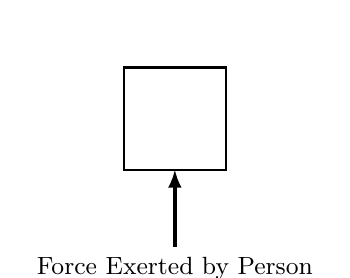
\begin{tikzpicture}[scale=1.3]
    \draw[thick] rectangle (1,1);
    \draw[very thick,->] (.5,-.75)--(.5,0) node[pos=0,below]{
      \small Force Exerted by Person};
  \end{tikzpicture}
\end{center}

\begin{questions}
  \question A person exerts an upward force on a box, as shown on the left. The
  box may be moving upward, downward, or not at all while the person exerts the
  upward force. For which of the following motions of the box is the work done
  by the person on the box correctly indicated?
  
  \begin{tabular}{clc}
    & Motion of Box & Work Done by Person on Box \\
    \hline
    (A) & No motion                  & Positive \\
    (B) & Upward, decreasing speed   & Negative \\
    (C) & Downward, constant speed   & Zero     \\
    (D) & Downward, increasing speed & Negative
  \end{tabular}
  
  %\uplevel{
  %  \centering
  %  \pic{.5}{spring-block}
  %}
  %\question A block is held at rest against a compressed spring at point $A$ at
  %the top of a frictionless track of height $h$, as shown above. The block is
  %released, loses contact with the spring at point $B$, and slides along the
  %track until it passes point $C$, also at height $h$. How do the potential
  %energy $U$ of the block-Earth system and the kinetic energy $K$ of the block
  %at point $C$ compare with those at point $A$?
  %
  %\begin{tabular}{ccc}
  %  & Potential Energy of Block-Earth System & Kinetic Energy of Block\\
  %  \hline
  %  (A) & $U_C=U_A$ & $K_C=K_A$ \\
  %  (B) & $U_C=U_A$ & $K_C>K_A$ \\
  %  (C) & $U_C>U_A$ & $K_C=K_A$ \\
  %  (D) & $U_C>U_A$ & $K_C>K_A$
  %\end{tabular}  

  \uplevel{
    \centering
    \pic{.4}{IMG_20200810_093039201}
  }
  \question A car with a \SI{500}{\newton} driver goes over a hill that has a
  radius of \SI{50}{\metre} as shown in the figure above. The velocity of the
  car is \SI{20}{\metre\per\second}. What are the approximate force and
  direction that the car exerts on the driver?
  \begin{choices}
    \choice\SI{900}\newton, up
    \choice\SI{400}\newton, down
    \choice\SI{100}\newton, up
    \choice\SI{500}\newton, up
  \end{choices}
  \newpage
  
  \uplevel{
    \pic{.35}{downpour}
  }
  \question\vspace{-.2in}An open cart on a level surface is rolling without
  frictional loss through a vertical downpour of rain, as shown above. As the
  cart rolls, an appreciable amount of rainwater accumulates in the cart. The
  speed of the cart will
  \begin{choices}
    \choice increase because of conservation of momentum
    \choice increase because of conservation of energy
    \choice decrease because of conservation of momentum
    \choice decrease because of conservation of energy
  \end{choices}

  \question Three forces at on an object. If the object is in translational
  equilibrium, which of the following must be true?
  \begin{enumerate}[nosep,leftmargin=18pt,label={\Roman*.}]
  \item The vector sum of the three forces must be equal to zero
  \item The magnitudes of the three forces must be equal
  \item All three forces must be parallel
  \end{enumerate}
  \begin{choices}
    \choice I only
    \choice II only
    \choice I and III only
    \choice II and III only
    \choice I, II and III
  \end{choices}
  
  \uplevel{
    \pic{.5}{spring-block}
  }
  \question A block is held at rest against a compressed spring
  at point $A$ at the top of a frictionless track of height $h$, as shown
  above. The block is released, loses contact with the spring at point $B$, and
  slides along the track until it passes point $C$, also at height $h$. How do
  the potential energy $U$ of the block-Earth system and the kinetic energy $K$
  of the block at point $C$ compare with those at point $A$?
  
  \begin{tabular}{ccc}
    & Potential Energy of Block-Earth System & Kinetic Energy of Block\\
    \hline
    (A) & $U_C=U_A$ & $K_C=K_A$ \\
    (B) & $U_C=U_A$ & $K_C>K_A$ \\
    (C) & $U_C>U_A$ & $K_C=K_A$ \\
    (D) & $U_C>U_A$ & $K_C>K_A$
  \end{tabular}

  \uplevel{
    \vspace{-.25in}
    \pic{.38}{impulses}
  }
  \question\vspace{-.3in} Objects X and Y are constrained to move along a
  straight line. The
  graphs above show the net force exerted along that line on each of the
  objects as functions of time. Which of the following correctly ranks the
  change in momentum $\Delta p$ of the objects?
  \begin{choices}
    \choice $\Delta p_X < \Delta p_Y$
    \choice $\Delta p_X = \Delta p_Y$ 
    \choice $\Delta p_X > \Delta p_Y$
    \choice The ranking cannot be determined without knowing the masses
    of the objects.
  \end{choices}
  
  \uplevel{
    \pic{.55}{car-collision}
  }
  \question\vspace{-.25in}In the setup shown above, a student uses motion
  detector 1 to measure the speed $\varv_i$ of a cart with mass $m$ before it
  collides with and sticks to a stationary cart with mass $M$. Motion detector
  2 measures the speed $\varv_f$ of the carts after the collision. The student
  repeats the experiment several times using different values of $\varv_i$ and
  creates a graph of $\varv_f$ as a function of $\varv_i$. The slope of this
  graph is most nearly equal to
  \begin{choices}
    \choice$\dfrac mM$
    \choice$\dfrac m{M+m}$
    \choice$\dfrac{M-m}{M+m}$
    \choice$\sqrt{\dfrac m{M+m}}$
  \end{choices}
  \newpage
  
  \uplevel{
    \pic{.7}{circular-arc}
    \vspace{-.2in}\textbf{Questions \ref{first}--\ref{last}:} The figures above
    show a small block of mass \SI{.20}{\kilo\gram} on a track in the shape of
    a circular arc. The block is released from rest at a height $H$ above the
    floor, as shown in Figure 1. The block slides along the track with
    negligible friction and leaves it at a height of \SI{.40}{\metre} above the
    floor and a speed of \SI{3.0}{\metre\per\second} at a \ang{30} angle, as
    shown in Figure 2.
  }

  \question The height $H$ is most nearly
  \begin{choices}
    \choice 0.45 m
    \choice 0.51 m
    \choice 0.86 m
    \choice 1.7 m
  \end{choices}
  \label{first}
    
  \question The magnitude of the gravitational force exerted on the block is
  $F_g$, and the magnitude of the normal force exerted by the track on the
  block is $F_n$. Which of the following correctly compares the magnitudes of
  these two forces when the block is at the lowest point on the track?
  \begin{choices}
    \choice $F_n>F_g$
    \choice $F_n=F_g$
    \choice $F_n<F_g$
    \choice The magnitudes cannot be compared without knowing the radius of the
    arc of the track.
  \end{choices}
    
  \question After the block leaves the track, what is the block's speed when it
  reaches the highest point of its motion?
  \begin{choices}
    \choice 0\hspace{.3in}
    \choice\SI{1.5}{\metre\per\second}\hspace{.3in} 
    \choice\SI{2.6}{\metre\per\second}\hspace{.3in}
    \choice\SI{3.0}{\metre\per\second}
  \end{choices}
  \label{last}
  
  \question Two satellites are in circular orbits around Earth. Satellite 1 has
  mass $m_0$ and an orbital radius of $2R_E$, where $R_E$ is the radius of
  Earth. Satellite 2 has mass $2m_0$ and an orbital radius of $3R_E$. Which of
  the following correctly compares the magnitude $F$ of the force exerted by
  Earth on each satellite and the speed $v$ of each satellite?

  \begin{tabular}{ccc}
    & Force & Speed\\ \hline
    (A) & $F_1>F_2$ & $\varv_1>\varv_2$ \\
    (B) & $F_1>F_2$ & $\varv_2>\varv_1$ \\
    (C) & $F_2>F_1$ & $\varv_1>\varv_2$ \\
    (D) & $F_2>F_1$ & $\varv_2>\varv_1$
  \end{tabular}

  \newpage
  \uplevel{
    \centering
    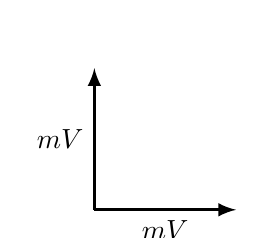
\begin{tikzpicture}[scale=1.8,very thick,->]
      \draw (0,0)--(0,1) node[midway,left]{$mV$};
      \draw (0,0)--(1,0) node[midway,below]{$mV$};
    \end{tikzpicture}
  }
  \question A stationary object explodes, breaking into three pieces of masses
  $m$, $m$ and $3m$. The two pieces of mass $m$ move off at right angles to each
  other with the same magnitude of momentum $mV$, as shown in the diagram
  above. What are the magnitude and direction of the velocity of the piece
  having mass $3m$?
  \label{last-mcq}
  \begin{tabular}{ccc}
    & Magnitude & Direction \\
    \hline
    (A) & $\dfrac V{\sqrt3}$  & {\Huge $\nearrow$} \\
    (B) & $\dfrac V{\sqrt3}$  & {\Huge $\swarrow$} \\
    (C) & $\dfrac{\sqrt2V}3$ & {\Huge $\nearrow$} \\
    (D) & $\dfrac{\sqrt2V}3$ & {\Huge $\swarrow$} \\
    (E) & $\sqrt2V$ & {\Huge $\swarrow$}
  \end{tabular}
  \newpage
  
  \uplevel{
    \centering
    \textbf{AP PHYSICS 1 PRACTICE TEST \#2\\
    SECTION 2: FREE-RESPONSE QUESTIONS\\
    4 QUESTIONS\\
    Time: 60 MINUTES}
  
    \vspace{.6in}
    \pic{.55}{bumper-cars}
  }
  \question[10] Several students are riding in bumper cars at an amusement
  park. The combined mass of car $A$ and its occupants is \SI{250}{\kilo\gram}.
  The combined mass of car $B$ and its occupants is \SI{200}{\kilo\gram}. Car
  $A$ is \SI{15}{\metre} away from car $B$ and moving to the right at
  \SI{2.0}{\metre\per\second}, as shown, when the driver decides to bump into
  car $B$, which is at rest.
  \begin{parts}
    \part Car $A$ accelerates at \SI{1.5}{\metre\per\second\squared} to a speed
    of \SI{5.0}{\metre\per\second} and then continues at constant velocity until
    it strikes car $B$. Calculate the total time for car $A$ to travel the
    \SI{15}\metre.
    \vspace{\stretch1}

    \uplevel{
      After the collision, car $B$ moves to the right at a speed of
      \SI{4.8}{\metre\per\second}.
    }
    \part Calculate the speed of car $A$ after the collision.
    \vspace{\stretch1}
    
    \part Indicate the direction of motion of car $A$ after the collision.

    \vspace{.1in}
    \underline{\hspace{.4in}} To the left\hspace{.3in}
    \underline{\hspace{.4in}} To the right\hspace{.3in}
    \underline{\hspace{.4in}} None; car $A$ is at rest.
    \vspace{\stretch1}

    \part Is this an elastic collision? Justify your answer.
    \vspace{\stretch1}
    
%    \vspace{.1in}
%    \underline{\hspace{.7in}} Yes\hspace{.3in}
%    \underline{\hspace{.7in}} No
  \end{parts}
  \newpage

  \uplevel{
    \centering
    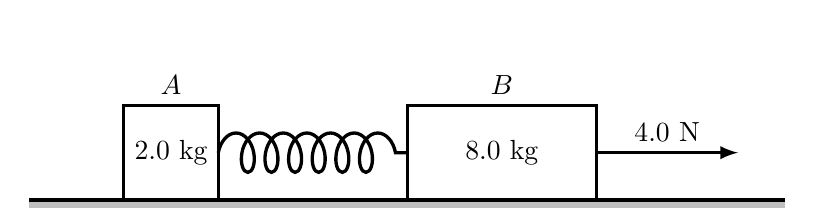
\begin{tikzpicture}[scale=1.2,very thick]
      \fill[gray!50] rectangle(8,-.2);
      \draw (0,0)--(8,0);
      \draw (1,0) rectangle(2,1) node[midway]{2.0 kg};
      \node[above] at (1.5,1){$A$};
      \draw (4,0) rectangle(6,1) node[midway]{8.0 kg};
      \node[above] at (5,1){$B$};
      \draw[->] (6,.5)--(7.5,.5) node[midway,above]{4.0 N};
      \draw[decoration={aspect=.6,segment length=3mm,amplitude=2.5mm,coil},
        decorate] (2,.5)--(4,.5);
    \end{tikzpicture}
  }
  
  \question[15] Block $A$ of mass \SI{2.0}{\kilo\gram} and block $B$ of mass
  \SI{8.0}{\kilo\gram} are connected as shown above by a spring of spring
  constant \SI{80}{\newton\per\metre} and negligible mass. The system is being
  pulled to the right across a horizontal frictionless surface by a horizontal
  force of \SI{4.0}\newton, as shown, with both blocks experiencing equal
  constant acceleration.
  \begin{parts}
    \part Calculate the force that the spring exerts on the \SI{2.0}{\kilo\gram}
    block.
    \vspace{\stretch1}
    
    \part Calculate the extension of the spring.
    \vspace{\stretch1}
    
    \uplevel{
      The system is now pulled to the left, as shown below, with both blocks
      again experiencing equal constant acceleration.
      \begin{center}
        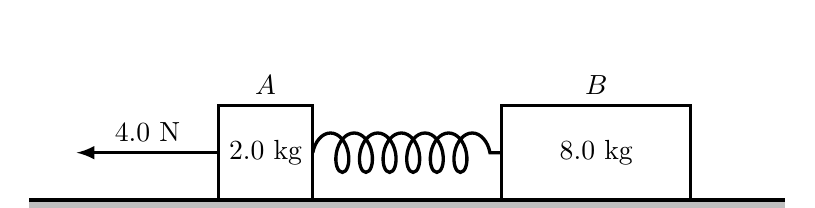
\begin{tikzpicture}[scale=1.2,very thick]
          \fill[gray!50] (-1,0) rectangle(7,-.2);
          \draw (-1,0)--(7,0);
          \draw (1,0) rectangle(2,1) node[midway]{2.0 kg};
          \node[above] at (1.5,1){$A$};
          \draw (4,0) rectangle(6,1) node[midway]{8.0 kg};
          \node[above] at (5,1){$B$};
          \draw[->] (1,.5)--(-.5,.5) node[midway,above]{4.0 N};
          \draw[decoration={aspect=.6,segment length=3mm,amplitude=2.5mm,coil},
            decorate] (2,.5)--(4,.5);
        \end{tikzpicture}
      \end{center}
    }
    
    \part Is the magnitude of the acceleration greater than, less than, or the
    same as before? Justify your answer.

    \vspace{.1in}
    \underline{\hspace{.4in}} Greater
    \underline{\hspace{.4in}} Less
    \underline{\hspace{.4in}} The same
    \vspace{\stretch1}
    
    \part Is the amount the spring has stretched greater than, less than, or
    the same as before? Justify your answer.

    \vspace{.1in}
    \underline{\hspace{.4in}} Greater
    \underline{\hspace{.4in}} Less
    \underline{\hspace{.4in}} The same
    \vspace{\stretch1}

    \part In a new situation, the blocks and spring are moving together at a
    constant speed of \SI{.50}{\metre\per\second} to the left. Block $A$ then
    hits and sticks to a wall. Calculate the maximum compression of the spring.
    \vspace{\stretch1}
  \end{parts}
  \newpage

%  \uplevel{
%    \pic{.35}{pulley-a-b}
%  }
%  \question[15] A rope of negligible mass passes over a pulley of negligible
%  mass attached to the ceiling, as shown above. One end of the rope is held by
%  Student $A$ of mass \SI{70}{\kilo\gram}, who is at rest on the floor. The
%  opposite end of the rope is held by Student $B$ of mass \SI{60}{\kilo\gram},
%  who is suspended at rest above the floor.
%  \begin{parts}
%    \part On the dots below that represent the students, draw and label
%    free-body diagrams showing the forces on Student $A$ and on Student $B$.
%
%    \vspace{.3in}
%    \begin{center}
%      \begin{tikzpicture}
%        \fill circle(.08) node[right]{$\;A$};
%        \fill (1,2.5) circle(.08) node[right]{$\;B$};
%      \end{tikzpicture}
%    \end{center}
%    \vspace{.3in}
%    
%    \part Calculate the magnitude of the force exerted by the floor on Student
%    $A$.
%    
%    \uplevel{
%      Student $B$ now climbs up the rope at a constant acceleration of
%      \SI{.25}{\metre\per\second\squared} with respect to the floor.
%    }
%    
%    \part Calculate the tension in the rope while Student B is accelerating.
%
%    \part As Student $B$ is accelerating, is Student $A$ pulled upward off the
%    floor? Justify your answer.
%
%    \part With what minimum acceleration must Student $B$ climb up the rope to
%    lift Student $A$ upward off the floor?  
%  \end{parts}
%  \newpage

  \uplevel{
    \pic{.66}{energy}
  }
  \question[15] Block $A$ of mass \SI{4.0}{\kilo\gram} is on a horizontal,
  frictionless tabletop and is placed against a spring of negligible mass and
  spring constant \SI{650}{\newton\per\metre}. The other end of the spring is
  attached to a wall. The block is pushed toward the all until the spring has
  been compressed a distance $x$, as shown above. The block is released and
  follows the trajectory shown, falling \SI{.80}{\metre} vertically and
  striking a target on the floor that is a horizontal distance of
  \SI{1.2}{\metre} from the edge of the table. Air resistance is negligible.
  \begin{parts}
    \part Calculate the time elapsed from the instant block $A$ leaves the
    table to the instant it strikes the floor.
    \vspace{\stretch1}
    
    \part Calculate the speed of the block as it leaves the table.
    \vspace{\stretch1}
    
    \part Calculate the distance $x$ the spring was compressed.
    \vspace{\stretch1}
    \newpage
    
    \uplevel{
      Block $B$, also of mass \SI{4.0}{\kilo\gram}, is now placed at the edge of
      the table. The spring is again compressed a distance $x$, and block $A$
      is released. As it nears the end of the table, it instantaneously
      collides with and sticks to block $B$. The blocks follow the trajectory
      shown in the figure below and strike the floor at a horizontal distance
      $d$ from the edge of the table.
      \pic{.66}{energy2}
    }

    \part Calculate $d$ if $x$ is equal to the value determined in part (c).
    \vspace{\stretch1}
    
    \part Consider the system consisting of the spring, the blocks, and the
    table. How does the total mechanical energy $E_2$ of the system just before
    the blocks leave the table compare to the total mechanical energy $E_1$ of
    the system just before block $A$ is released? Justify your answer.

    \vspace{.1in}
    \underline{\hspace{.4in}} $E_2<E_1$\hspace{.3in}
    \underline{\hspace{.4in}} $E_2=E_1$\hspace{.3in}
    \underline{\hspace{.4in}} $E_2>E_1$
    \vspace{\stretch1}
  \end{parts}
  \newpage
  
  \uplevel{
    \centering
    \pic{.5}{plunger}
  }
  \question[7] Identical blocks 1 and 2 are placed on a horizontal surface at
  points A and E, respectively, as shown. The surface is frictionless except
  for the region between points C and D, where the surface is rough. Beginning
  at time $t_A$, block 1 is pushed with a \underline{constant} horizontal force
  from point A to point B by a mechanical plunger. Upon reaching point B, block
  1 loses contact with the plunger and continues moving to the right along the
  horizontalsurface toward block 2. Block 1 collides with and sticks to block 2
  at point E, after which the two-block system continues moving across the
  surface, eventually passing point F. On the axes below, sketch the speed of
  the center of mass of the two-block system as a function oftime, from time
  $t_A$ until the blocks pass point F at time $t_F$. The times at which block 1
  reaches points Athrough F are indicated on the time axis.
  \uplevel{
    \centering
    \begin{tikzpicture}[scale=1.3]
      \draw[->,thick] (0,0)--(12,0) node[midway,below=15]{Time};
      \draw[->,thick] (0,0)--(0,5.5)
      node[pos=.8,left=10,rotate=90]{Speed of Center of Mass};
      \foreach \x in {2,3,4.3,6.3,10.5}
      \draw[dashed,thick,gray] (\x,0)--+(0,5.3);
      \fill circle (.06) node[below]{$t_A$} node[left]{$0$};
      \fill (2,0) circle (.06) node[below]{$t_B$};
      \fill (3,0) circle (.06) node[below]{$t_C$};
      \fill (4.3,0) circle (.06) node[below]{$t_D$};
      \fill (6.3,0) circle (.06) node[below]{$t_E$};
      \fill (10.5,0) circle (.06) node[below]{$t_C$};
      \foreach \y in {1,...,5} \draw[dashed,thick,gray] (0,\y)--+(11,0);
    \end{tikzpicture}
  }
\end{questions}
\end{document}
